\documentclass[10pt]{hackr26}
% hackr26.cls is not in the repo. Page count was checked with a stand-in class
% (article, 10pt, 1in margins). It must be rechecked on the real template.

% Source files (all under tips/Wylie_SmallestCircle/ unless noted). No Sources table
% exists for this task, so `% src:` comments name the file and section directly.
%   study_tips.html        reviewed page: theorem, dispatcher (Fig. 5), case table (Table 1)
%   review_study_tips.md   review and Fix log (corrected claims)
%   01_study_guide.md      background and references
%   02_possible_solutions.md  derivations, verification plan V1-V4
%   03_plan_and_design.md  paper structure and page budget
%   problems/Wylie_SmallestCircle.pdf  problem statement
%   experiments/smallest_circle/  run 150312_v2_n1000: results/summary.json, results/rows.csv,
%     manifest.json, README.md (criteria), CHANGELOG.md (v2 row)

\usepackage{tikz}
\usepackage{booktabs,tabularx,array}
\usepackage{float}
\usetikzlibrary{calc,arrows.meta}

%----------------------- Macros and Definitions --------------------------
\newcommand{\dist}{\operatorname{dist}}
\newcommand{\R}{\mathbb{R}}
\setlength{\textfloatsep}{3pt plus 1pt minus 2pt}
\setlength{\floatsep}{3pt plus 1pt minus 2pt}
\setlength{\intextsep}{3pt plus 1pt minus 2pt}
\setlength{\abovecaptionskip}{3pt}\setlength{\belowcaptionskip}{0pt}

%----------------------- Title -------------------------------------------
\title{The Smallest Circle Touching Three Lines in 3D}

\author{
    Taek Lim
    \thanks{University of Texas Rio Grande Valley.}
}

\index{Lim, Taek}
\date{}

%------------------------------ Text -------------------------------------
\begin{document}
\maketitle
\small\setlength{\baselineskip}{10pt}
\begin{abstract}
We solve Tim Wylie's problem of the smallest circle in $\R^3$ that touches three lines.
It is a great circle of a smallest ball that meets all three lines.
An $O(1)$ test decides whether two or three lines are active.
We give closed forms for 10 of the 16 cases of the problem's Figure~1.
For the other 6, only the two-active subcase is closed.
A numerical solver agrees wherever a closed form exists.
\end{abstract}

%%%%%%%%%%%%%%%%%%%%%%%%%%%%%%%%%%%%%%%%%%%%%%%%%%%%%%%%%%%%%%%%%%%%%%%%%%%%%%%%%%%%
\section{Introduction} \label{sec:intro}
Given three lines in $\R^3$, we want the circle of smallest radius that touches all of them (UTRGV Research Hackathon 2026, Tim Wylie).
We return its center $c$, radius $r$ and plane normal $n$, for all positions in the problem's Figure~1.
% src: problems/Wylie_SmallestCircle.pdf p.1
The ball subproblem is the intersection radius problem~\cite{BJMR94}.
We add the circle-to-ball reduction, an active-line test and closed forms.
We read ``touch'' as ``intersect'': the circle curve shares a point with each line.
We do not treat the tangent reading.
% src: owner decision 2026-11-07, study_tips.html Step 6 "touch" pitfall, review_study_tips.md M3
A line is $L_i=\{a_i+t\,d_i\}$ with $|d_i|=1$, and $P_i=I-d_id_i^{\top}$.
The distance from $c$ to $L_i$ is $\dist_i(c)=|P_i(c-a_i)|$, and the foot is $q_i=a_i+((c-a_i)\cdot d_i)\,d_i$.
% src: study_tips.html Step 1 (papers tab), 02_possible_solutions.md notation block

%%%%%%%%%%%%%%%%%%%%%%%%%%%%%%%%%%%%%%%%%%%%%%%%%%%%%%%%%%%%%%%%%%%%%%%%%%%%%%%%%%%%
\section{Main Theorem} \label{sec:thm}
Let $f(c)=\max_i \dist_i(c)$ and $r^*=\min_c f(c)$.
The ball $B(c^*,r^*)$ is a smallest ball that meets all three lines.

\begin{lemma}[Lower bound]\label{lem:lower}
A circle with center $c$ and radius $r$ that touches all three lines has $r\ge f(c)\ge r^*$.
\end{lemma}
\begin{proof}
Let $p_i$ be a common point of the circle and $L_i$. Then $\dist_i(c)\le |c-p_i|=r$.
\end{proof}
% src: study_tips.html Step 1 "Lower bound" box; 02_possible_solutions.md Lemma 1

\begin{lemma}[Attainment]\label{lem:attain}
Some $c^*$ attains $r^*$, and a great circle of $B(c^*,r^*)$ touches all three lines.
\end{lemma}
\begin{proof}
Each $\dist_i$ is a norm of an affine map, so $f$ is convex.
If two lines are not parallel, $f\to\infty$ at infinity and a minimizer exists. If all are parallel, we reduce to the cross-section.
If $r^*=0$, the circle is the common point of the lines.
Let $r^*>0$ and $u_i=(c^*-q_i)/r^*$.
Line $i$ is \emph{active} if $\dist_i(c^*)=r^*$.
By the subdifferential of a maximum of convex functions, $0\in\operatorname{conv}\{u_i: i\text{ active}\}$.
The active $u_i$ are unit vectors, so at least two lines are active.

\emph{Three active.} The $u_i$ are coplanar, so the feet $q_i=c^*-r^*u_i$ lie in a plane through $c^*$, which gives a great circle.

\emph{Two active, $i$ and $j$.} Then $u_i=-u_j$, so $q_i,q_j$ are antipodal.
Since $\dist_k(c^*)\le r^*$ and $L_k$ is unbounded, $L_k$ meets the sphere at some $s$.
The plane through $q_i,q_j,s$ contains the diameter $q_iq_j$, hence $c^*$.
\end{proof}
% src: study_tips.html Step 1 theorem box; review_study_tips.md B.1 (KKT, antipodal), m2, m4; 02_possible_solutions.md Lemma 2

\begin{theorem}\label{thm:main}
The smallest touching circle has radius $r^*$ and is a great circle of a smallest ball meeting all three lines.
\end{theorem}
\begin{proof}
Lemma~\ref{lem:lower} gives $r\ge r^*$, and Lemma~\ref{lem:attain} attains it.
A circle of radius $r^*$ about $c'$ needs $f(c')\le r^*$, so $c'$ minimizes $f$.
\end{proof}
% src: review_study_tips.md B.1 row "세 직선이면 최소 원 = 최소 구의 대원"


\paragraph{Dispatcher.}
For each pair $(i,j)$ let $\rho_{ij}=\dist(L_i,L_j)/2$.
Let $C_{ij}$ (a point, midline or line) be the centers of the smallest ball meeting $L_i,L_j$.
Take the largest $\rho_{ij}$, with third line $L_k$.
If the largest value is tied, test every tied pair.
If $\dist(C_{ij},L_k)\le\rho_{ij}$, two lines are active, $r=\rho_{ij}$, and $c\in C_{ij}$ is nearest to $L_k$.
The plane holds the diameter $q_iq_j$ and a point $s\in L_k$ on the sphere (Lemma~\ref{lem:attain}).
Otherwise three are active (Table~\ref{tab:cases}).
The test is closed form and $O(1)$.
% src: study_tips.html Step 4 flow (Fig. 5) and review_study_tips.md B.1 "흐름도: 최대 ρ 쌍 하나만 검사"

\begin{lemma}[Dispatcher]\label{lem:disp}
If every pair with the largest $\rho$ fails the test, three lines are active.
If a pair passes, $r^*=\rho_{ij}$.
\end{lemma}
\begin{proof}
Let only $i,j$ be active. Then $u_i=-u_j$, so $q_j-q_i=2(c^*-q_i)$.
This vector is normal to $d_i$ and $d_j$, so $q_iq_j$ is the common perpendicular.
Hence $2r^*=\dist(L_i,L_j)$, that is, $r^*=\rho_{ij}$.
Also $r^*\ge\rho_{kl}$ for every pair, so $\rho_{ij}$ is the largest.
Further $c^*\in C_{ij}$, and $\dist(C_{ij},L_k)\le\dist_k(c^*)\le r^*=\rho_{ij}$, so the pair passes.
The contrapositive is the first claim.
If a pair passes, a ball of radius $\rho_{ij}$ meets all three lines, so $r^*\le\rho_{ij}\le r^*$.
\end{proof}
% src: review_paper.md 4.4 (proof copied, not re-derived)

\begin{figure}[!t]
\centering
\begin{minipage}[t]{0.45\linewidth}
\centering
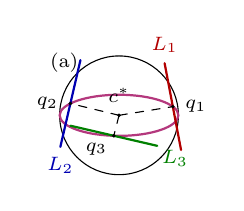
\begin{tikzpicture}[scale=0.58, >=Stealth, line cap=round, font=\scriptsize]
  \draw (0,0) circle (1.3);
  \draw[thick, magenta!70!black] (0,0) ellipse (1.3 and 0.45);
  \coordinate (q1) at ({1.3*cos(25)},{0.45*sin(25)});
  \coordinate (q2) at ({1.3*cos(145)},{0.45*sin(145)});
  \coordinate (q3) at ({1.3*cos(265)},{0.45*sin(265)});
  \draw[dashed] (0,0) -- (q1);
  \draw[dashed] (0,0) -- (q2);
  \draw[dashed] (0,0) -- (q3);
  \draw[red!70!black, thick] ($(q1)+(0.18,-0.95)$) -- ($(q1)+(-0.18,0.95)$) node[above] {$L_1$};
  \draw[blue!70!black, thick] ($(q2)+(0.22,0.95)$) -- ($(q2)+(-0.22,-0.95)$) node[below] {$L_2$};
  \draw[green!50!black, thick] ($(q3)+(-0.95,0.22)$) -- ($(q3)+(0.95,-0.22)$) node[below right=-2pt] {$L_3$};
  \fill (0,0) circle (1.2pt) node[above=1pt] {$c^*$};
  \fill (q1) circle (1.2pt) node[right=1pt] {$q_1$};
  \fill (q2) circle (1.2pt) node[left=1pt] {$q_2$};
  \fill (q3) circle (1.2pt) node[below left=-1pt] {$q_3$};
\node at (-1.2,1.15) {(a)};
\end{tikzpicture}
\end{minipage}\hfill
\begin{minipage}[t]{0.53\linewidth}
\centering
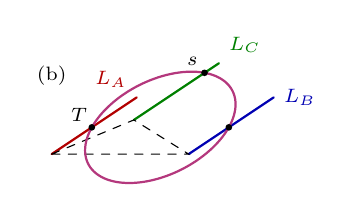
\begin{tikzpicture}[x={(0.58cm,0cm)}, y={(0.3cm,0.2cm)}, z={(0cm,0.62cm)}, >=Stealth, line cap=round, font=\scriptsize]
  % lines along y: A=(-1.5,.,0), B=(1.5,.,0), C=(0.3,.,0.7)
  \draw[red!70!black, thick]   (-1.5,-1.7,0)   -- (-1.5,1.9,0)   node[above left] {$L_A$};
  \draw[blue!70!black, thick]  (1.5,-1.7,0)    -- (1.5,1.9,0)    node[right] {$L_B$};
  \draw[green!50!black, thick] (0.3,-1.7,0.7)  -- (0.3,1.9,0.7)  node[above right] {$L_C$};
  % cross-section triangle T, obtuse at C
  \draw[dashed] (-1.5,-1.7,0) -- (1.5,-1.7,0) -- (0.3,-1.7,0.7) -- cycle;
  \node at (-0.9,-1.7,0.8) {$T$};
  % tilted circle: diameter AB, passes through s on L_C
  \draw[thick, magenta!70!black, domain=0:360, samples=60, smooth, variable=\t]
    plot ({1.5*cos(\t)}, {1.319*sin(\t)}, {0.715*sin(\t)});
  \fill (-1.5,0,0) circle (1.2pt);
  \fill (1.5,0,0) circle (1.2pt);
  \fill (0.3,1.292,0.7) circle (1.2pt) node[above left=-1pt] {$s$};
\node at (-1.5,-1.7,1.6) {(b)};
\end{tikzpicture}
\end{minipage}
\caption{(a) Smallest ball, great circle. (b) Obtuse 3-parallel case. Why: the plane may be tilted.}
\label{fig:geom}
\end{figure}
% src: study_tips.html Figures 1, 2 (schematic, coordinates chosen for drawing only)

%%%%%%%%%%%%%%%%%%%%%%%%%%%%%%%%%%%%%%%%%%%%%%%%%%%%%%%%%%%%%%%%%%%%%%%%%%%%%%%%%%%%
\section{Case Analysis} \label{sec:cases}
Symbols in Table~\ref{tab:cases}: ``$n$ meet'' counts intersection points, as in the problem's Figure~1.
$\delta$ is the distance of a skew pair, and a parallel pair has gap $w=2h$ and midline $M$.
We put a parallel pair $L_1,L_2$ at $x=\mp h$, $z=0$, along $y$, and write $L_3=\{a_3+t\,e\}$.
A \emph{perpendicular} line is normal to the plane of two meeting or parallel lines and meets it at $S$.
For a skew pair it is parallel to their common perpendicular.
For lines crossing at $P$ with angle $\theta$, $b$ is the bisector toward $S$ and $v=S-P$.
Also $q(z)=\min_y\dist_3^2-z^2$, with $z$ the height of $c$ above the parallel pair's plane.
% src: study_tips.html Step 5 "표의 기호" box

\begin{table}[!t]
\centering
\scriptsize
\renewcommand{\arraystretch}{1.0}
\setlength{\tabcolsep}{2.5pt}
\setlength{\aboverulesep}{0pt}\setlength{\belowrulesep}{0pt}
\begin{tabularx}{\linewidth}{>{\raggedright\arraybackslash}p{3.25cm} >{\centering\arraybackslash}p{0.8cm} X >{\raggedright\arraybackslash}p{1.2cm}}
\toprule
Case & Active & Answer: $c$, $r$, plane & Status\\
\midrule
3 meet (triangle $ABC$) & 3 &
Incircle, in the triangle's plane. $c=(\ell_aA+\ell_bB+\ell_cC)/(\ell_a+\ell_b+\ell_c)$, $r=2\,\mathrm{Area}/(\ell_a+\ell_b+\ell_c)$, with $\ell_a=|BC|$ etc. & closed\\
\midrule
Concurrent or coincident (not in problem Fig.~1) & 0 or 2 & Concurrent: $r=0$, $c=P$, a point circle. Coincident: two lines, $r$ is half their distance. & closed\\
\midrule
2 meet, 1 cross & 2 or 3 &
If the line meeting both passes within $\delta/2$ of the midpoint $m$ of the skew pair's common perpendicular: $c=m$, $r=\delta/2$. Otherwise three are active (open). & 2-active closed\\
\midrule
1 meet, 2 cross (over, over/under) & 2 or 3 &
Dispatcher decides. Label: side of the meeting pair's plane on which $L_3$ passes. & 2-active closed\\
\midrule
0 meet (all skew) & 2 or 3 &
Two active: dispatcher. Three active (open): quadrics $|P_i(c-a_i)|^2=r^2$ and the cubic $\det[q_1-c,q_2-c,q_3-c]=0$. Bézout bound 24 in the unknowns $(c,r)$. The system is even in $r$, so at most 12 solutions have $r>0$. & 2-active closed\\
\midrule
2 parallel, 1 meets both or 1 meet 1 cross & 2 & $r=w/2$. For ``meets both'', $c$ is any point of $M$ within $w/2$ of the transversal. & closed\\
\midrule
2 parallel, 0 meet (over, over/under) & 2 or 3 &
Dispatcher first. If $(L_1,L_2)$ has the largest $\rho$ and $\dist(M,L_3)\le h$, then $r=h$. If another pair has the largest $\rho$ and passes, then $r$ is its $\rho$. If three are active, $x=0$ and $r^2=h^2+z^2$. Here $z$ is the root of $q(z)=Az^2+Bz+C=h^2$ of smallest $|z|$. With $k=e_xa_{3,z}-e_za_{3,x}$ and $D=1-e_y^2$: $A=-e_z^2/D$, $B=-2e_xk/D$, $C=k^2/D$. & closed\\
\midrule
3 parallel, coplanar & 2 & $r$ is half the gap of the outer two lines. $c$ is any point of their midline. & closed\\
\midrule
3 parallel, 2 coplanar (prism) & 3 or 2 &
Cross-section triangle $T$. Acute: circumcircle of $T$, plane $\perp$ lines. Right or obtuse: $r=$ longest side$/2$, plane tilted (our Fig.~\ref{fig:geom}b). & closed\\
\midrule
1 meet + perpendicular & 2 or 3 &
3 active: $c=P+tb$, $r=t\sin(\theta/2)$, $t$ = smaller root of $t^2\cos^2(\theta/2)-2t\,(b\cdot v)+|v|^2=0$. & closed\\
\midrule
1 cross + perpendicular & 2 or 3 &
A $180^\circ$ rotation swapping $L_1,L_2$ may remain. If $S$ is on its axis, $c$ is on the axis and $\dist_1^2=\dist_3^2$ is a one-variable quadratic. Else use the dispatcher. & 2-active closed\\
\midrule
2 parallel + perpendicular & 2 &
Between the lines: $r=w/2$, $c$ not unique. Outside: take $S$ at $x=x_S>h$. The far line and $L_3$ are active: $r=(x_S+h)/2$, $x_c=(x_S-h)/2$, plane $z=0$. & closed\\

\bottomrule
\end{tabularx}
\caption{Cases of the problem's Figure~1 and two more. 2-active closed: the three-active subcase is open.}
\label{tab:cases}
\end{table}
% src: study_tips.html Step 5 table (Table 1) and Fix log in review_study_tips.md (M1, M2, m4, m8, m10, m13, m15); 02_possible_solutions.md sections A-F

%%%%%%%%%%%%%%%%%%%%%%%%%%%%%%%%%%%%%%%%%%%%%%%%%%%%%%%%%%%%%%%%%%%%%%%%%%%%%%%%%%%%
% src: study_tips.html Figures 1 and 2; 02_possible_solutions.md section C2


%%%%%%%%%%%%%%%%%%%%%%%%%%%%%%%%%%%%%%%%%%%%%%%%%%%%%%%%%%%%%%%%%%%%%%%%%%%%%%%%%%%%
\section{Verification and Open Problems} \label{sec:ver}
We compared Table~\ref{tab:cases} with a second-order cone program (SOCP), $\min r$ s.t.\ $|P_i(c-a_i)|\le r$.
The inputs were 20 presets and 1,000 random instances per case (18 cases, seed 20261107).
An instance passes if three values are at most $10^{-6}$: the relative error $|r_{\mathrm{closed}}-r_{\mathrm{socp}}|/\max(1,r_{\mathrm{socp}})$, the touch residual, and the excess of the center over $r_{\mathrm{socp}}$.
The code (commit 6337385) ran on the Cradle cluster.
A first run exposed an unstable plane normal for coincident lines, fixed in v2.
All 18 cases pass, with 0 closed-form failures and 0 solver failures.
The largest relative error is $9.0\times10^{-9}$ and the largest touch residual is $2.6\times10^{-10}$.
The solver returned optimal on 18,015 of 18,020 rows, and the other 5 solved on a retry at tolerance $10^{-8}$.
Verification covers only inputs with a closed form, 14,833 of 18,020 rows.
The other 3,187 rows have no closed form and ran on the SOCP only.
Closed-form coverage: 296/1,002 (2 meet, 1 cross), 446/1,001 (1 meet, over), 216/1,001 (1 meet, over/under), 289/1,002 (all skew, 713 SOCP only), 573/1,001 (skew perpendicular).
% src: experiments/smallest_circle/runs/150312_v2_n1000/results/summary.json (overall, counts, scaled_dr max, touch_max max); results/rows.csv (socp_status counts, status counts); manifest.json (seed, tolerances, code_commit, job); README.md (criteria, inputs); CHANGELOG.md (v2 finding 1); repo CLAUDE.md (Cradle)
\paragraph{Open problems and future work.}
The general skew case with three active lines is open.
Its eliminant degree and Galois group decide whether radicals suffice, as for the 12 common tangents of four unit balls~\cite{MPT01}.
We leave that degree to future work.
Theorem~\ref{thm:main} fails for four lines, e.g.\ lines through the vertices of an inscribed regular tetrahedron, each perpendicular to its radius.
Its center is optimal with $r^*=R$, but the touch points are not coplanar.
% src: study_tips.html Step 5 (0 meet row), papers tab (Macdonald-Pach-Theobald, Phillips-Schou 2025 row (claim dropped, space)), Step 4 future work; review_study_tips.md m5; review_paper.md 4.6

\paragraph{AI usage.}
Claude (Anthropic) assisted with literature, derivations, figures and drafting.


%---------------------------- Bibliography -------------------------------
\scriptsize
\setlength{\parskip}{0pt}
\begin{thebibliography}{9}
\setlength{\itemsep}{0pt}
\bibitem{BJMR94} B.~K. Bhattacharya et al. Optimal algorithms for some intersection radius problems. \emph{Computing}, 52(3), 1994.
\bibitem{MPT01} I.~G. Macdonald, J.~Pach, and T.~Theobald. Common tangents to four unit balls in $\R^3$. \emph{Discrete Comput. Geom.}, 26(1), 2001.
\end{thebibliography}

\end{document}
